%%%%%%%%%%%%%%%%%%%%%%%%%%%%%%%%%%%%%%%%%%%%%%%%%%%%%%%%%%
\documentclass[xcolor=pdftex,dvipsnames,table,10pt]{beamer}
%handout, if no \pause

\usepackage{tabularx}
\usepackage{tikz}
\usepackage[]{algorithm2e}
\usepackage{listings}
\usepackage{lstautogobble}
\usepackage{graphicx}
\usepackage{hyperref}
\usepackage{amsmath}
\usepackage{xcolor}
\usepackage{subfigure}
\usepackage[style=authoryear,backend=biber,mincitenames=1,maxcitenames=2, uniquelist=false]{biblatex}
\bibliography{fossilDating.bib}

\newcommand{\Mstrict}{{M1}}
\newcommand{\Mrelaxed}{{M8}}
% turnover = birth / death
\newcommand{\turnover}{\nu}

% sampling proportion = \psi / \psi + \mu
\newcommand{\fosp}{s}
\newcommand{\sampleprop}{sampling proportion}


\definecolor{newblue}{rgb}{0.3, 0.5, 0.9}
\definecolor{newblue1}{rgb}{0.3, 0.3, 0.7}
\definecolor{newred}{RGB}{200,0,0}

%\documentclass[handout,xcolor=pdftex,dvipsnames,table]{beamer} % USE THIS WITH pdfpages STUFF
%\usepackage{pgfpages}
%\pgfpagesuselayout{resize to}[a4paper, landscape]

\definecolor{headerColour}{RGB}{180, 230, 245}
\definecolor{headerTitleColour}{RGB}{0, 60, 80}
\definecolor{sectionShadedColour}{RGB}{50, 110, 130}
\definecolor{subsectionHighlightColour}{RGB}{50, 50, 50}
\definecolor{subsectionShadedColour}{RGB}{100, 100, 100}

\setbeamercolor{subsection in sidebar}{fg=subsectionHighlightColour}
\setbeamercolor{subsection in sidebar shaded}{fg=subsectionShadedColour}
\setbeamercolor{structure}{fg=headerTitleColour, bg=headerColour}
\setbeamercolor{title}{fg=headerTitleColour, bg=white}
\setbeamercolor{section in sidebar shaded}{fg=sectionShadedColour}

\usetheme{Goettingen}
\makeatletter\setbeamertemplate{sidebar canvas \beamer@sidebarside}[vertical shading][top=headerColour,bottom=white]\makeatother

%% to suppress subsections in sidebar:
%\setbeamertemplate{subsection in sidebar shaded}
%{\vspace*{-\baselineskip}}
%\setbeamertemplate{subsubsection in sidebar shaded}
%{\vspace*{-\baselineskip}}

\usepackage{amsmath, amssymb}
\usepackage{fancyvrb}


% Font modification
\usefonttheme{professionalfonts}
\usepackage{cmbright}
\usepackage{eulervm}
\newfont{\Ss}{cmcsc12 scaled 1600}

% no navigation symbols at the bottom of frames
\beamertemplatenavigationsymbolsempty
\setbeamertemplate{footline}[frame number] 

\usepackage{multirow} % allows entries across multipe rows in tables
\usepackage{booktabs} % makes fancier rulers in tables
%\usepackage{setspace} % spacing between lines

%%%%%%%%%%%%%%%%%%
%% Bibliography related stuff:
% control space between lines
  \let\oldthebibliography=\thebibliography
  \let\endoldthebibliography=\endthebibliography
  \renewenvironment{thebibliography}[1]{
    \begin{oldthebibliography}{#1}
      \setlength{\parskip}{-0.5ex}
      \setlength{\itemsep}{-0.5ex}
  }{ \end{oldthebibliography} }
% Force entry to be in one line
\setbeamertemplate{bibliography entry title}{}
\setbeamertemplate{bibliography entry location}{}
\setbeamertemplate{bibliography entry note}{}
% Set bullet point shape:
\setbeamertemplate{bibliography item}{-}
%%%%%%%%%%%%%%


\newenvironment{items}{\begin{list}{$\bullet$}{\itemsep0ex plus 0.2ex
\parsep0ex plus 0.2ex \topsep0ex \parskip0ex}}{\end{list}}
\newcommand{\head}[1]
{\slide{\begin{center}\textbf{#1}\vspace*{-0.5\baselineskip}
{\color{red}\rule{\textwidth}{1mm}}\end{center}}}
\parskip0.3ex

\newcommand{\cT}{{\mathcal T}}


%\defbeamertemplate*{title page}{customized}[1][]
%{
%  \titlepage
%  \usebeamerfont{title}\inserttitle\par
%  \usebeamerfont{subtitle}\usebeamercolor[fg]{subtitle}\insertsubtitle\par
%  \bigskip
%  \usebeamerfont{author}\insertauthor\par
%  \usebeamerfont{institute}\insertinstitute\par
%  \usebeamerfont{date}\insertdate\par
%  \usebeamercolor[fg]{titlegraphic}\inserttitlegraphic
%}


\title[Total-evidence dating]{`Total-evidence' Bayesian estimation of phylogeny, divergence times and fossil ages}
\author[]{Alexei Drummond�}
\date{The Royal Society, London \\ 9th November 2015}
\institute{Professor of Computational Biology \\ Department of Computer Science \\ University of Auckland}
%\titlegraphic{\hspace*{8cm}\includegraphics[height=1.5cm]{figures/cEvo_logo_transparent.png}}
%{\small Link to Script\&Slides:  \url{http://www.tb.ethz.ch/education} 
%}

%%%%%%%%%%%%%% Figure caption setup
\usepackage[compatibility=false]{caption}
\captionsetup[figure]{labelsep=space,justification=centering}
\renewcommand{\figurename}{\scriptsize Figure adapted from}

% syntax: \figureCaption{Citation caption}{Second (real) caption}
% second caption can be skipped, first one has to be suppressed if you want to skip it
\newcommand\figureCaption[2]{%
  \captionsetup{aboveskip=0.1cm,belowskip=0cm}
  \caption{\scriptsize #1}
  \caption*{#2}
}

%%%%%%%%%%%%%% Fixme and comment setup�
\definecolor{red}{HTML}{C92D39}
\definecolor{green}{HTML}{498A44}

% syntax: \fixme{What needs to be fixed}
\newcommand{\fixme}[1]{\textcolor{red}{\texttt{{\bf FIX ME:} #1}}}
% Hide all fixmes by switching the line above to this:
%\newcommand{\fixme}[1]{}

% syntax: \comment{Name of commenter}{C omment}
\newcommand{\comment}[2]{\textcolor{green}{{\bf Comment by {#1}}: #2}}
% Hide all comments by switching the line above to this:
%\newcommand{\comment}[2]{}

\begin{document}

%Slide1
\frame{\titlepage}

%%%%%%%%%%%%%%%%%%%%%%%%%%%%%%%%%%%%%%%%%%%%%%
\section{Fossilized birth-death process}
%%%%%%%%%%%%%%%%%%%%%%%%%%%%%%%%%%%%%%%%%%%%%%

\begin{frame}{The problem}

\begin{itemize}

\item We have 
\begin{itemize}
  \item \normalsize{{\bf molecular data} of extant species,} 
  \item \normalsize{{\bf morphological data} of extant and fossil species and }
  \item \normalsize{{\bf Fossil ages} (or geological time intervals).}
\end{itemize} 
\item We want to utilise all this data to learn about {\bf evolutionary history} and {\bf macroevolutionary processes}.
\item {\bf Bayesian statistical inference} is our preferred method of learning about the world.


\end{itemize}

\end{frame}


%%%%%%%%%%%%%%%%%%%%%%%%%%%%%%%%%%%%%%%%%%%%%%


\begin{frame}{Node dating}

\begin{itemize}
\item {\bf Divergence time dating is tricky :) }
\item {\bf A common practice is node dating}. One or more divergences in a phylogeny are assigned ages by identifying fossils of known geological age that correspond* to each divergence. 
\item This method has a few drawbacks:
\begin{itemize}
\item Often only the oldest fossil in a calibrated clade is used,
\item Calibration densities are often {\it ad hoc},
\item Difficult* to combine calibrations with tree priors,
\item Computational complexity of some methods mean that only a few nodes can be calibrated (Heled \& Drummond 2012).
\end{itemize}
\end{itemize}

\end{frame}


%%%%%%%%%%%%%%%%%%%%%%%%%%%%%%%%%%%%%%%%%%%%%%


\begin{frame}{Tip dating and total evidence}

Two main features of new method for divergence-time dating:
\begin{itemize}
\item Explicit modelling of fossilization events as a part of the tree branching process (Pyron 2011, Heath {\it et al} 2014),
\item Utilising all existing data \textcolor{newblue1}{(total evidence)} in a joint inference (Pyron 2011, Ronquist {\it et al} 2012).
\end{itemize}

\end{frame}


%%%%%%%%%%%%%%%%%%%%%%%%%%%%%%%%%%%%%%%%%%%%%%


%\begin{frame}{Total evidence}

%\begin{itemize}

%\item Pyron 2011 uses Lewis MK model to model evolution of morphological characters.  
%\item Ronquist et al 2012, Wood et al 2012. 
%\item They used Yule or Uniform tree prior. 
%\end{itemize}


%\end{frame}
 

%%%%%%%%%%%%%%%%%%%%%%%%%%%%%%%%%%%%%%%%%%%%%%


\begin{frame}{Birth-death-sampling models}

\begin{figure}
  \begin{center}
               \usetikzlibrary{shapes,snakes}

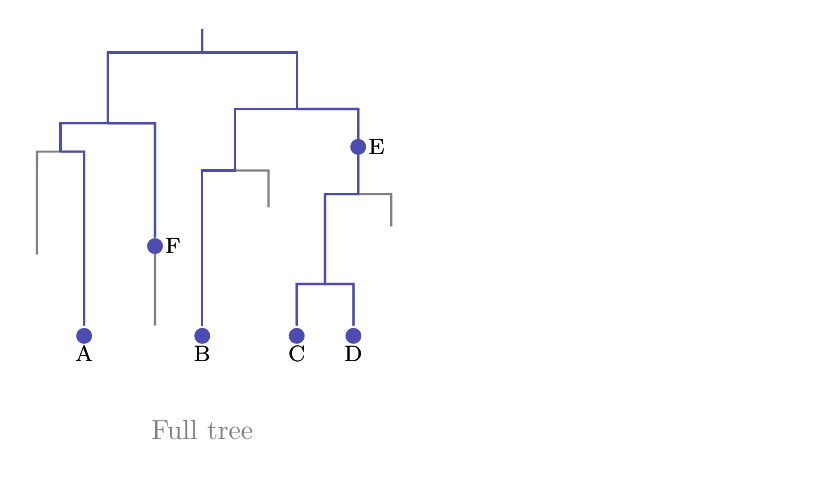
\begin{tikzpicture}[thick, scale=0.6, color=gray]

\begin{scope}

%terminal nodes
\node at (-3.5, 2.5)(s2){};
\node at (0, 1)(s3){};
\node at (-2.5, 1)(s4){};
\node at (4, 3.1)(s5){};
\node at (1.4, 3.5)(s7){};
\node at (-1, 1)(s8){};
\node at (3.2, 1)(s9){};
\node at (2, 1)(s10){};

%branches
\draw (0, 7.5) -- (0,7) -- (-2, 7) --(-2, 5.5) --(-3, 5.5) -- (-3, 4.9) -- (-3.5, 4.9) -- (s2);
\draw (-3, 4.9) -- (-2.5, 4.9) -- (s4); 
\draw (-2, 5.5) -- (-1, 5.5) -- (s8); 
\draw (0,7) -- (2,7) -- (2,5.8) -- (0.7, 5.8) -- (0.7, 4.5) -- (0, 4.5) -- (s3); 
\draw (0.7, 4.5) -- (1.4, 4.5) -- (s7); 
\draw (2, 5.8) -- (3.3, 5.8) -- (3.3, 4) -- (2.6, 4) -- (2.6, 2.1) -- (2, 2.1) -- (s10); 
\draw (2.6, 2.1) -- (3.2, 2.1) -- (s9);
\draw (3.3, 4) -- (4, 4) -- (s5);

\node at (0, -1) {Full tree};

\pause 

%sampled nodes
\node[fill,circle, inner sep=2pt] at (-2.5, 1)(sA){};
\node[anchor=north] (Alet) at (sA) {\textcolor{black}{\footnotesize A}};
\node[fill,circle, inner sep=2pt] at (0, 1)(sB){};
\node[anchor=north] (Alet) at (sB) {\textcolor{black}{\footnotesize B}};
\node[fill,circle, inner sep=2pt] at (2, 1)(sC){};
\node[anchor=north] (Alet) at (sC) {\textcolor{black}{\footnotesize C}};
\node[fill,circle, inner sep=2pt] at (3.2, 1)(sD){};
\node[anchor=north] (Alet) at (sD) {\textcolor{black}{\footnotesize D}};

\pause 

\node[fill,circle, inner sep=2pt] at (3.3, 5)(sE){};
\node[anchor=west] (Alet) at (sE) {\textcolor{black}{\footnotesize E}};
\node[fill,circle, inner sep=2pt] at (-1, 2.9)(sF){};
\node[anchor=west] (Alet) at (sF) {\textcolor{black}{\footnotesize F}};

\pause 

\color{newblue1}

%branches
\draw (0, 7.5) -- (0,7) -- (-2, 7) --(-2, 5.5) --(-3, 5.5) -- (-3, 4.9);
\draw (-3, 4.9) -- (-2.5, 4.9) -- (s4); 
\draw (-2, 5.5) -- (-1, 5.5) -- (sF); 
\draw (0,7) -- (2,7) -- (2,5.8) -- (0.7, 5.8) -- (0.7, 4.5) -- (0, 4.5) -- (s3); 
\draw (2, 5.8) -- (3.3, 5.8) -- (3.3, 4) -- (2.6, 4) -- (2.6, 2.1) -- (2, 2.1) -- (s10); 
\draw (2.6, 2.1) -- (3.2, 2.1) -- (s9);

%sampled nodes
\node[fill,circle, inner sep=2pt] at (-2.5, 1)(sA){};
\node[anchor=north] (Alet) at (sA) {\textcolor{black}{\footnotesize A}};
\node[fill,circle, inner sep=2pt] at (0, 1)(sB){};
\node[anchor=north] (Alet) at (sB) {\textcolor{black}{\footnotesize B}};
\node[fill,circle, inner sep=2pt] at (2, 1)(sC){};
\node[anchor=north] (Alet) at (sC) {\textcolor{black}{\footnotesize C}};
\node[fill,circle, inner sep=2pt] at (3.2, 1)(sD){};
\node[anchor=north] (Alet) at (sD) {\textcolor{black}{\footnotesize D}};

\node[fill,circle, inner sep=2pt] at (3.3, 5)(sE){};
\node[anchor=west] (Alet) at (sE) {\textcolor{black}{\footnotesize E}};
\node[fill,circle, inner sep=2pt] at (-1, 2.9)(sF){};
\node[anchor=west] (Alet) at (sF) {\textcolor{black}{\footnotesize F}};

\end{scope}

\begin{scope}[xshift=8.5cm]

\color{white}

%terminal nodes
\node[fill,circle, inner sep=2pt] at (-3, 1)(sA){};
\node[anchor=north] (Alet) at (sA) {\textcolor{white}{\footnotesize A}};
\node[fill,circle, inner sep=2pt] at (0.7, 1)(sB){};
\node[anchor=north] (Alet) at (sB) {\textcolor{white}{\footnotesize B}};
\node[fill,circle, inner sep=2pt] at (2.7, 1)(sC){};
\node[anchor=north] (Alet) at (sC) {\textcolor{white}{\footnotesize C}};
\node[fill,circle, inner sep=2pt] at (3.9, 1)(sD){};
\node[anchor=north] (Alet) at (sD) {\textcolor{white}{\footnotesize D}};
\node[fill,circle, inner sep=2pt] at (-1, 2.9)(sF){};
\node[anchor=west] (Alet) at (sF) {\textcolor{white}{\footnotesize F}};
\node[fill,circle, inner sep=2pt] at (3.3, 5)(sE){};
\node[anchor=west] (Alet) at (sE) {\textcolor{white}{\footnotesize E}};

%branches
\draw (0, 7.5) -- (0,7) -- (-2, 7) --(-2, 5.5) --(-3, 5.5)  -- (sA);
\draw (-2, 5.5) -- (-1, 5.5) -- (sF); 
\draw (0,7) -- (2,7) -- (2,5.8) -- (0.7, 5.8) -- (0.7, 4.5) -- (sB); 
\draw (2, 5.8) -- (3.3, 5.8) -- (3.3, 4) -- (3.3, 2.1) -- (2.7, 2.1) -- (sC); 
\draw (3.3, 2.1) -- (3.9, 2.1) -- (sD);

\end{scope}

\end{tikzpicture}


            \end{center}
            
         \end{figure}    
\end{frame}


%%%%%%%%%%%%%%%%%%%%%%%%%%%%%%%%%%%%%%%%%%%%%% 


\begin{frame}{Birth-death-sampling models}


 \begin{figure}
            \begin{center}
               \usetikzlibrary{shapes,snakes}

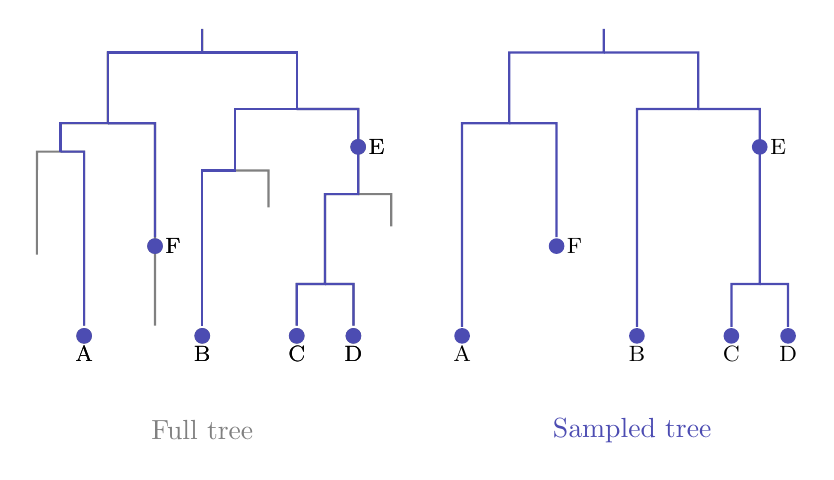
\begin{tikzpicture}[thick, scale=0.6, color=gray]

\begin{scope}

%terminal nodes
\node at (-3.5, 2.5)(s2){};
\node at (0, 1)(s3){};
\node at (-2.5, 1)(s4){};
\node at (4, 3.1)(s5){};
\node at (1.4, 3.5)(s7){};
\node at (-1, 1)(s8){};
\node at (3.2, 1)(s9){};
\node at (2, 1)(s10){};

%branches
\draw (0, 7.5) -- (0,7) -- (-2, 7) --(-2, 5.5) --(-3, 5.5) -- (-3, 4.9) -- (-3.5, 4.9) -- (s2);
\draw (-3, 4.9) -- (-2.5, 4.9) -- (s4); 
\draw (-2, 5.5) -- (-1, 5.5) -- (s8); 
\draw (0,7) -- (2,7) -- (2,5.8) -- (0.7, 5.8) -- (0.7, 4.5) -- (0, 4.5) -- (s3); 
\draw (0.7, 4.5) -- (1.4, 4.5) -- (s7); 
\draw (2, 5.8) -- (3.3, 5.8) -- (3.3, 4) -- (2.6, 4) -- (2.6, 2.1) -- (2, 2.1) -- (s10); 
\draw (2.6, 2.1) -- (3.2, 2.1) -- (s9);
\draw (3.3, 4) -- (4, 4) -- (s5);

\node at (0, -1) {Full tree};

%sampled nodes
\node[fill,circle, inner sep=2pt] at (-2.5, 1)(sA){};
\node[anchor=north] (Alet) at (sA) {\textcolor{black}{\footnotesize A}};
\node[fill,circle, inner sep=2pt] at (0, 1)(sB){};
\node[anchor=north] (Alet) at (sB) {\textcolor{black}{\footnotesize B}};
\node[fill,circle, inner sep=2pt] at (2, 1)(sC){};
\node[anchor=north] (Alet) at (sC) {\textcolor{black}{\footnotesize C}};
\node[fill,circle, inner sep=2pt] at (3.2, 1)(sD){};
\node[anchor=north] (Alet) at (sD) {\textcolor{black}{\footnotesize D}};
\node[fill,circle, inner sep=2pt] at (3.3, 5)(sE){};
\node[anchor=west] (Alet) at (sE) {\textcolor{black}{\footnotesize E}};
\node[fill,circle, inner sep=2pt] at (-1, 2.9)(sF){};
\node[anchor=west] (Alet) at (sF) {\textcolor{black}{\footnotesize F}};


\color{newblue1}

%branches
\draw (0, 7.5) -- (0,7) -- (-2, 7) --(-2, 5.5) --(-3, 5.5) -- (-3, 4.9);
\draw (-3, 4.9) -- (-2.5, 4.9) -- (s4); 
\draw (-2, 5.5) -- (-1, 5.5) -- (sF); 
\draw (0,7) -- (2,7) -- (2,5.8) -- (0.7, 5.8) -- (0.7, 4.5) -- (0, 4.5) -- (s3); 
\draw (2, 5.8) -- (3.3, 5.8) -- (3.3, 4) -- (2.6, 4) -- (2.6, 2.1) -- (2, 2.1) -- (s10); 
\draw (2.6, 2.1) -- (3.2, 2.1) -- (s9);

%sampled nodes
\node[fill,circle, inner sep=2pt] at (-2.5, 1)(sA){};
\node[anchor=north] (Alet) at (sA) {\textcolor{black}{\footnotesize A}};
\node[fill,circle, inner sep=2pt] at (0, 1)(sB){};
\node[anchor=north] (Alet) at (sB) {\textcolor{black}{\footnotesize B}};
\node[fill,circle, inner sep=2pt] at (2, 1)(sC){};
\node[anchor=north] (Alet) at (sC) {\textcolor{black}{\footnotesize C}};
\node[fill,circle, inner sep=2pt] at (3.2, 1)(sD){};
\node[anchor=north] (Alet) at (sD) {\textcolor{black}{\footnotesize D}};
\node[fill,circle, inner sep=2pt] at (3.3, 5)(sE){};
\node[anchor=west] (Alet) at (sE) {\textcolor{black}{\footnotesize E}};
\node[fill,circle, inner sep=2pt] at (-1, 2.9)(sF){};
\node[anchor=west] (Alet) at (sF) {\textcolor{black}{\footnotesize F}};


\end{scope}

\begin{scope}[xshift=8.5cm]

\color{newblue1}

%terminal nodes
\node[fill,circle, inner sep=2pt] at (-3, 1)(sA){};
\node[anchor=north] (Alet) at (sA) {\textcolor{black}{\footnotesize A}};
\node[fill,circle, inner sep=2pt] at (0.7, 1)(sB){};
\node[anchor=north] (Alet) at (sB) {\textcolor{black}{\footnotesize B}};
\node[fill,circle, inner sep=2pt] at (2.7, 1)(sC){};
\node[anchor=north] (Alet) at (sC) {\textcolor{black}{\footnotesize C}};
\node[fill,circle, inner sep=2pt] at (3.9, 1)(sD){};
\node[anchor=north] (Alet) at (sD) {\textcolor{black}{\footnotesize D}};
\node[fill,circle, inner sep=2pt] at (-1, 2.9)(sF){};
\node[anchor=west] (Alet) at (sF) {\textcolor{black}{\footnotesize F}};
\node[fill,circle, inner sep=2pt] at (3.3, 5)(sE){};
\node[anchor=west] (Alet) at (sE) {\textcolor{black}{\footnotesize E}};

%branches

\draw (0, 7.5) -- (0,7) -- (-2, 7) --(-2, 5.5) --(-3, 5.5)  -- (sA);
\draw (-2, 5.5) -- (-1, 5.5) -- (sF); 
\draw (0,7) -- (2,7) -- (2,5.8) -- (0.7, 5.8) -- (0.7, 4.5) -- (sB); 
\draw (2, 5.8) -- (3.3, 5.8) -- (3.3, 4) -- (3.3, 2.1) -- (2.7, 2.1) -- (sC); 
\draw (3.3, 2.1) -- (3.9, 2.1) -- (sD);

\node at (0.6, -1) {\textcolor{newblue1}{Sampled tree}};

\end{scope}

\end{tikzpicture}


            \end{center}
            
         \end{figure}
    
\end{frame}


%%%%%%%%%%%%%%%%%%%%%%%%%%%%%%%%%%%%%%%%%%%%%% 


\begin{frame} {Fossillized birth-death model (FBD)}


\begin{columns}[t]
\begin{column}{.5\textwidth}

Stadler 2010, Heath {\it et al} 2014. 
\vspace{0.2cm}

The process starts at time $t_{or}>0$ and ends at time zero (present time).  
  \vspace{0.01cm}
   \begin{itemize}
\item birth rate $\lambda$
\item death rate $\mu$
\item sampling rate $\psi$
\item sampling at present probability $\rho$ 
   \end{itemize}
\vspace{0.01cm}

   \end{column}
   \begin{column}{.5\textwidth}

            \begin{center}
               \usetikzlibrary{shapes,snakes}

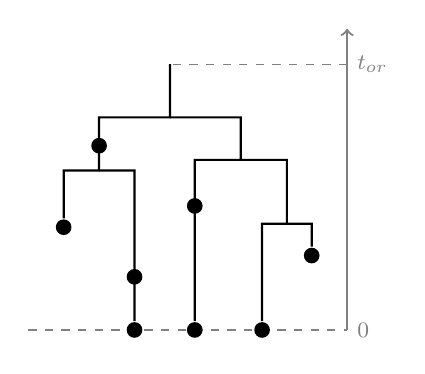
\begin{tikzpicture}[thick,scale=0.45]

\begin{scope}

\draw[ -> ,color=gray] (5, 1) -- (5, 9.5);
\draw[thin,dashed,color=gray] (5, 8.5) -- (0, 8.5);

\node[anchor=west]  at (5, 8.5) (or) {\textcolor{gray}{\footnotesize $t_{or}$}};

\draw[thin,dashed, color=gray] (-4, 1) -- (5, 1);
\node[anchor=west]  at (5, 1) (zero) {\textcolor{gray}{\footnotesize $0$}};



%sampled nodes
\node[fill,circle, inner sep=2pt] at (-3, 3.9)(s2){};
\node[fill,circle, inner sep=2pt] at (0.7, 4.5)(s1){};
\node[fill,circle, inner sep=2pt] at (0.7, 1)(s3){};
\node[fill,circle, inner sep=2pt] at (-2, 6.2)(s4){};
\node[fill,circle, inner sep=2pt] at (4, 3.1)(s5){};
\node[fill,circle, inner sep=2pt] at (-1, 1)(s8){};
\node[fill,circle, inner sep=2pt] at (-1, 2.5)(s9){};
\node[fill,circle, inner sep=2pt] at (2.6, 1)(s10){};


%branches
\draw (0, 8.5) -- (0,7) -- (-2, 7) --(-2, 5.5) --(-3, 5.5) -- (-3, 4.9) -- (s2);
\draw (-2, 5.5) -- (-1, 5.5) -- (s8); 
\draw (0,7) -- (2,7) -- (2,5.8) -- (0.7, 5.8) -- (0.7, 4.5) -- (s3); 
\draw (2, 5.8) -- (3.3, 5.8) -- (3.3, 4) -- (2.6, 4) --  (s10); 
\draw (3.3, 4) -- (4, 4) -- (s5);



\end{scope}



\end{tikzpicture}




            \end{center}
         
         \begin{center}\emph{Sampled tree} \end{center}   

   \end{column}    
\end{columns}

\vspace{0.2cm}

Model parameters: \color{newblue1} $\eta = (t_{or}, \lambda, \mu, \psi, \rho)$.

\color{black}
All the parameters are identifiable. 

\vspace{1.5cm}


\end{frame}


%%%%%%%%%%%%%%%%%%%%%%%%%%%%%%%%%%%%%%%%%%%%%%


\begin{frame} {Fossilized birth-death (FBD) skyline model}

Stadler \& K\"uhnert et al 2012, Gavryushkina {\it et al} 2014.

\vspace{0.2cm}

There are $k$ time intervals and parameters remain constants within the intervals but may vary from one interval to another

\begin{columns}[c]
\begin{column}{.5\textwidth}
\begin{itemize}
\item birth rates $\lambda_1, \ldots, \lambda_k$
\item death rates $\mu_1, \ldots, \mu_k$
\item sampling rates $\psi_1, \ldots, \psi_k$
\item sampling at time $t_k$ (present) probability $\rho$
\end{itemize}

\begin{center}
Model parameters:
\color{newblue1} $\eta = (t_{or}, \bar \lambda, \bar \mu, \bar \psi, \rho)$ 

\end{center}
  \end{column}
   \begin{column}{.5\textwidth}
\begin{center}
\usetikzlibrary{shapes,snakes}

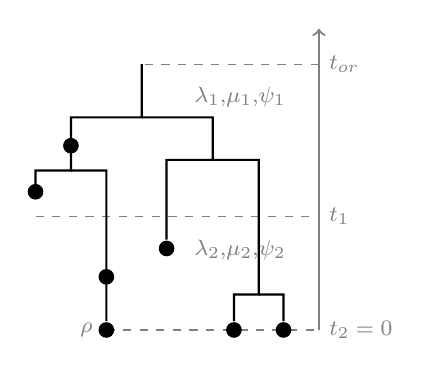
\begin{tikzpicture}[thick,scale=0.45]

\begin{scope}

\draw[ -> ,color=gray] (5, 1) -- (5, 9.5);
\draw[thin,dashed,color=gray] (5, 8.5) -- (0, 8.5);
\node[anchor=west]  at (5, 8.5) (or) {\textcolor{gray}{\footnotesize $t_{or}$}};

\draw[thin,dashed,color=gray] (-3, 4.2) -- (5, 4.2);
\node[anchor=west]  at (5, 4.2) (t1) {\textcolor{gray}{\footnotesize $t_1$}};


\draw[thin, dashed,color=gray] (-1, 1) -- (5, 1);
\node[anchor=west]  at (5, 1) (zero) {\textcolor{gray}{\footnotesize $t_2=0$}};

\node[anchor=south west]  at (1.2, 7.0) (y) {\textcolor{gray}{\footnotesize $\lambda_1$,$\mu_1$,$\psi_1$}};

\node[anchor=south west]  at (1.2, 2.7) (y) {\textcolor{gray}{\footnotesize $\lambda_2$,$\mu_2$,$\psi_2$}};

%\node[anchor=east]  at (-3.1, 4.2) (y) {\textcolor{gray}{\footnotesize $\rho_1$}};
\node[anchor=east]  at (-1.1, 1) (y) {\textcolor{gray}{\footnotesize $\rho$}};




%sampled nodes
\node[fill,circle, inner sep=2pt] at (-3, 4.9)(s2){};
\node[fill,circle, inner sep=2pt] at (0.7, 3.3)(s3){};
\node[fill,circle, inner sep=2pt] at (-2, 6.2)(s4){};
\node[fill,circle, inner sep=2pt] at (4, 1)(s5){};
\node[fill,circle, inner sep=2pt] at (-1, 1)(s8){};
\node[fill,circle, inner sep=2pt] at (-1, 2.5)(s9){};
\node[fill,circle, inner sep=2pt] at (2.6, 1)(s10){};


%branches
\draw (0, 8.5) -- (0,7) -- (-2, 7) --(-2, 5.5) --(-3, 5.5) -- (-3, 4.9) -- (s2);
\draw (-2, 5.5) -- (-1, 5.5) -- (s8); 
\draw (0,7) -- (2,7) -- (2,5.8) -- (0.7, 5.8) -- (0.7, 4.5) -- (s3); 
\draw (2, 5.8) -- (3.3, 5.8) -- (3.3, 2) -- (2.6, 2) --  (s10); 
\draw (3.3, 2) -- (4, 2) -- (s5);

\end{scope}



\end{tikzpicture}


\end{center}
\begin{center}\emph{\small Sampled tree} \end{center}   
 \end{column}    
\end{columns}

\end{frame}


%%%%%%%%%%%%%%%%%%%%%%%%%%%%%%%%%%%%%%%%%%%%%%

\iffalse 

\begin{frame}{Variation in the choice of the tree model parameters}

The $t_{or}$ parameter can be replaced with $t_{root}$ parameter assuming the process started with a branching event. 

\vskip2mm

Instead of $\lambda$, $\mu$, and $\psi$ we can also use an alternative parameterisation:

\renewcommand{\arraystretch}{1.2}

\begin{equation*} 
\begin{tabular}{ll} 
\text{net diversification rate} & $d = \lambda-\mu$  \\ 
\text{turnover rate} & $\turnover = \frac \mu \lambda$ \\ 
\text{\sampleprop} & $\fosp = \frac\psi {\mu + \psi}$  \\ 
\end{tabular} \end{equation*}

\end{frame}

\fi
%%%%%%%%%%%%%%%%%%%%%%%%%%%%%%%%%%%%%%%%%%%%%%


\begin{frame}{Heath {\it et al} approach and its extensions}

 Heath {\it et al} 2014 first used FBD model to infer divergence times of bears in a Bayesian MCMC framework:  

\begin{itemize}
\item The topology of extant species is fixed
\item Only used occurrence dates of fossils, and no morphology 
\item Fixed $\rho$ to the truth in the inference
\end{itemize}

We extend this model in two ways:

\begin{itemize}
\item Sampling sampled ancestor trees (Gavryushkina {\it et al} 2014)
\item Incorparating morphological data
\end{itemize}

Implemented in SA and Morph-models packages for BEAST2 (\url{www.beast2.org})

\end{frame}


%%%%%%%%%%%%%%%%%%%%%%%%%%%%%%%%%%%%%%%%%%%%%%


\begin{frame}{Comparative data of fossil tips vs only occurrence dates}

\begin{figure}
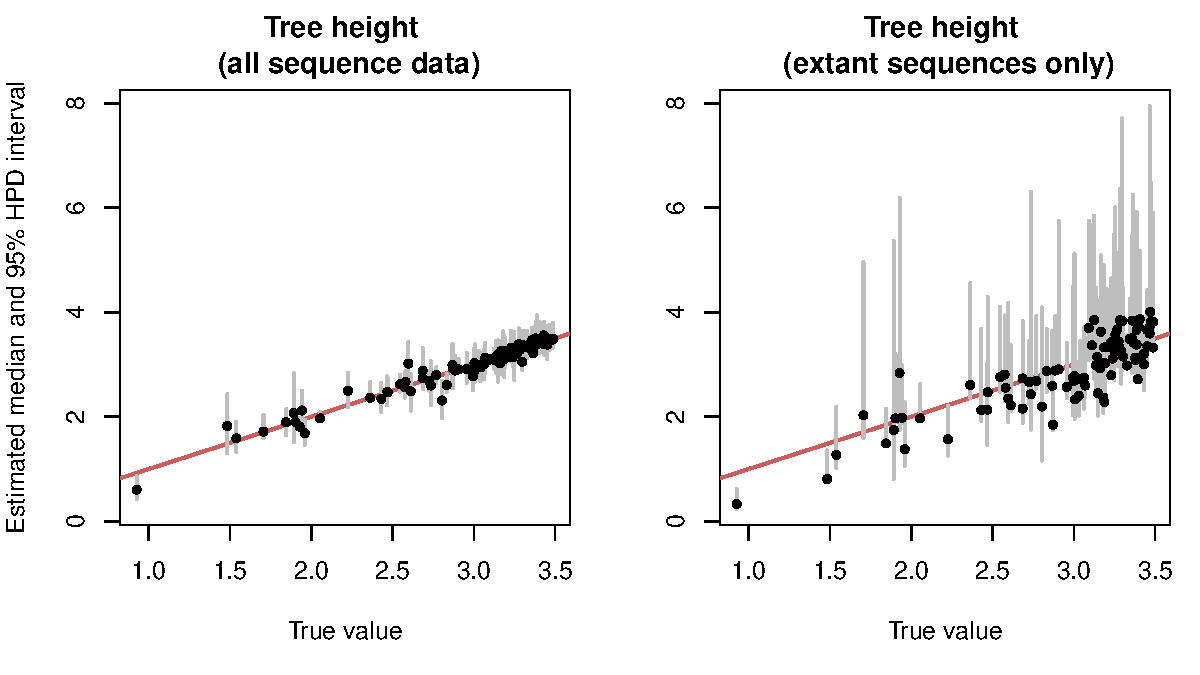
\includegraphics[width=\textwidth]{pics/Height_SA/Rplots.pdf}
\end{figure}

\end{frame}



%%%%%%%%%%%%%%%%%%%%%%%%%%%%%%%%%%%%%%%%%%%%%%


\begin{frame}{Comparative data of fossil tips vs only occurrence dates}

\setlength{\oddsidemargin}{0.1in} % adjust as necessary

\begin{columns}[c]

\begin{column}{.7\textwidth}
\begin{center}
\begin{figure}
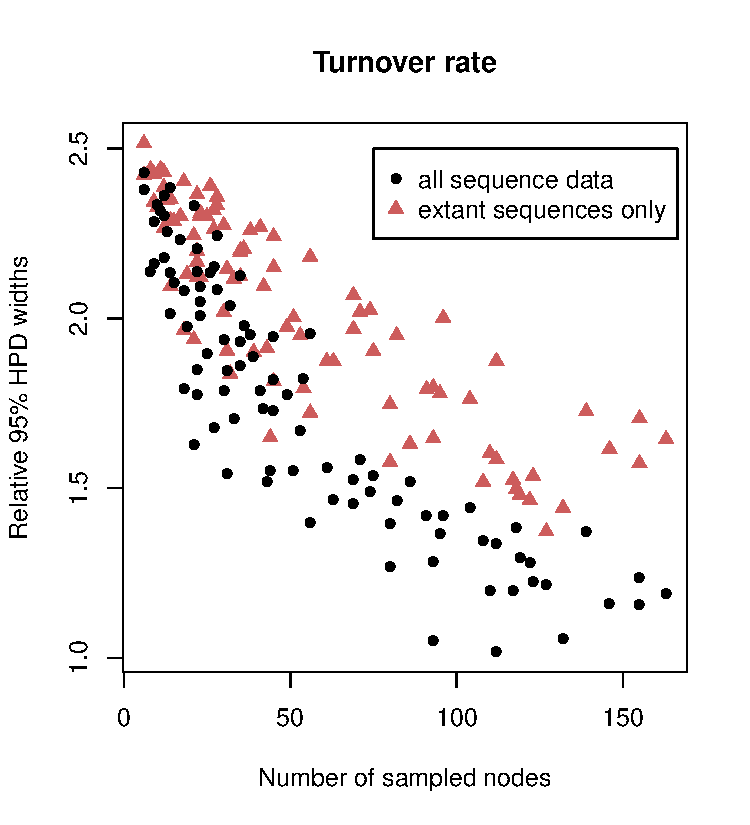
\includegraphics[height=0.65\textheight]{pics/TurnoverHPD/Rplots.pdf}
\end{figure}
\end{center}
 \end{column}
 
\begin{column}{.3\textwidth}
\begin{center}
turnover~rate~=~$\frac \mu \lambda$ 
\end{center}
 \end{column}    
\end{columns}

\end{frame}


%%%%%%%%%%%%%%%%%%%%%%%%%%%%%%%%%%%%%%%%%%%%%%


\begin{frame}{Biased estimates when not modelling sampled ancestors}

\begin{figure}
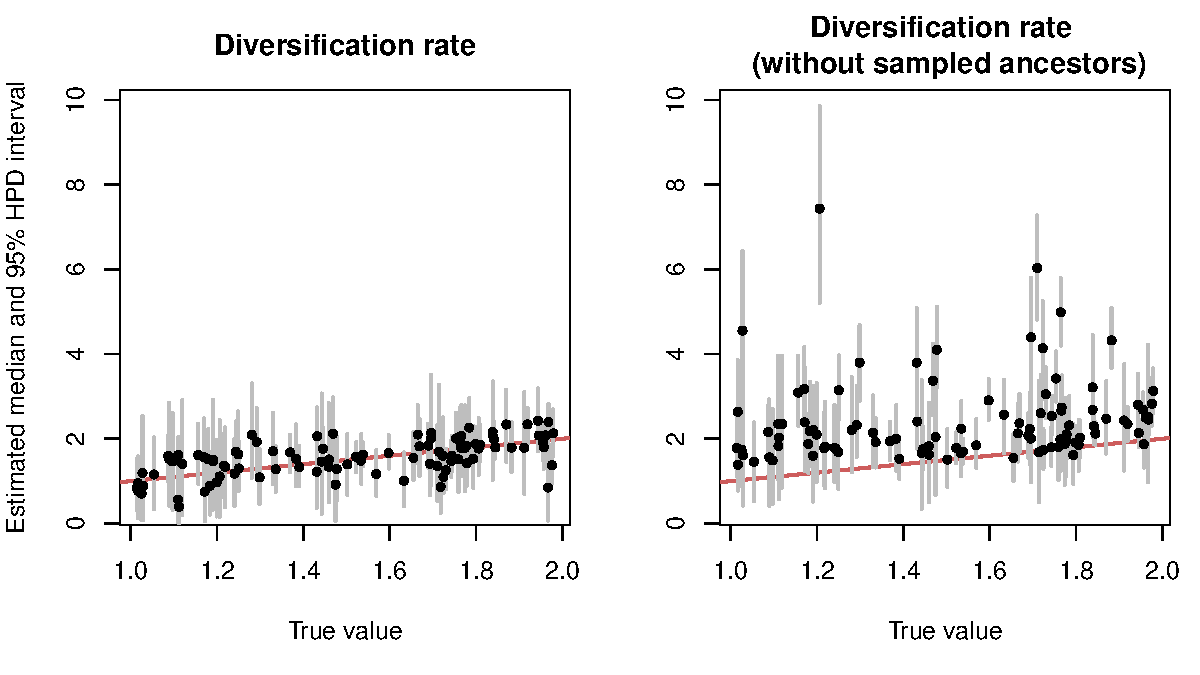
\includegraphics[width=\textwidth]{pics/SAvsNoSA/Rplots.pdf}
\end{figure}

\begin{center}
diversification rate = $\lambda-\mu$ 
\end{center}

\end{frame}

%%%%%%%%%%%%%%%%%%%%%%%%%%%%%%%%%%%%%%%%%%%%%%
\section{Penguin dating}
%%%%%%%%%%%%%%%%%%%%%%%%%%%%%%%%%%%%%%%%%%%%%%


\begin{frame}{Analysis of penguin morphological data}

Penguin dataset (Ksepka et al 2012) consisting of morphological data of:
\begin{itemize}
\item all extant penguins (19 species)
\item 36 fossil species assigned to stratigraphic intervals
\end{itemize}

\vskip2mm

Models:

\begin{itemize}
\item Lewis MK vs MKv (Lewis 2001)
\item Partitions vs single alignment
\item Rate variation across sites and across partitions
\item Tree prior: FBD and Skyline FBD
\item Different tree model parameterisations
\end{itemize}


\end{frame}


%%%%%%%%%%%%%%%%%%%%%%%%%%%%%%%%%%%%%%%%%%%%%%

\begin{frame}{Parameterisations}

\renewcommand{\arraystretch}{1.2}

lmp:

\color{newblue1} 

\begin{equation*} 
\begin{tabular}{ll} 
\text{birth rate} & $\lambda$  \\ 
\text{death rate} & $\mu$ \\ 
\text{sampling rate} & $\psi$  \\ 
\textcolor{black}{other parameters} & \textcolor{black}{$t_{or}, \rho$} \\
\end{tabular} \end{equation*}

\textcolor{black}{dvs:}

\begin{equation*} 
\begin{tabular}{ll} 
\text{net diversification rate} & $d = \lambda-\mu$  \\ 
\text{turnover rate} & $\turnover = \frac \mu \lambda$ \\ 
\text{\sampleprop} & $\fosp = \frac\psi {\mu + \psi}$  \\ 
\textcolor{black}{other parameters} & \textcolor{black}{$t_{or}, \rho$} \\
\end{tabular} \end{equation*}



\end{frame}

%%%%%%%%%%%%%%%%%%%%%%%%%%%%%%%%%%%%%%%%%%%%%%



\begin{frame}
\begin{figure}
\includegraphics[width=0.7\textwidth]{../../ag_morpho_data/figures/sa.pdf}
\label{saPostPr}
\end{figure}
\small{Probabilities of each fossil to be a sampled ancestor across models.

{\it P} stands for the partitioned model, {\it G} for gamma variation across sites, {\it Mkv} for conditioning on 
variable characters, {\it R} for relaxed clock model, {\it dns} for $d$, $\nu$, and $s$ tree prior parameterisation, {\it lmp} for $
\lambda$, $\mu$, and $\psi$ tree prior parameterisation.} 
\end{frame}

%%%%%%%%%%%%%%%%%%%%%%%%%%%%%%%%%%%%%%%%%%%%%%

\begin{frame}
\begin{figure}
\includegraphics[width=\textwidth]{../../ag_morpho_data/figures/pp.pdf}
\label{postPredictive}
\end{figure}
\small{The posterior and posterior predictive distributions for (left) tree length, $T$, and genealogical $D_F$ statistics and (right) $B_1$ tree imbalance statistic and Colless's tree imbalance index, $I_c$, for model 8. 

The posterior trees are on the unbalanced end of the predictive distribution.}
\end{frame}

%%%%%%%%%%%%%%%%%%%%%%%%%%%%%%%%%%%%%%%%%%%%%%

\begin{frame}
\begin{figure}
\includegraphics[width=\textwidth]{../../ag_morpho_data/figures/tree.pdf}
\label{penguinTree}
\end{figure}
\footnotesize{A maximum sampled ancestor clade credibility tree for the total-evidence analysis. % with mean node ages. 
The numbers in blue show the posterior supports of clades. The filled red and black circles represent sampled 
ancestors. Fossils with positive evidence of being sampled ancestors are shown in red.}

\end{frame}

%%%%%%%%%%%%%%%%%%%%%%%%%%%%%%%%%%%%%%%%%%%%%%

\begin{frame}
\begin{figure}
\begin{center}
\includegraphics[width=0.75\textwidth]{../../ag_morpho_data/figures/BayesFactors.pdf}
\label{fig:BF}
\end{center}
\end{figure}
\small{The evidence fossil sampled ancestors. The samples above the shaded area have positive evidence to be sampled ancestors and below the shaded area have positive evidence to be terminal nodes.}

\end{frame}

%%%%%%%%%%%%%%%%%%%%%%%%%%%%%%%%%%%%%%%%%%%%%%

\begin{frame}
\begin{figure}
\includegraphics[width=0.95\textwidth]{../../ag_morpho_data/figures/extant_tree.pdf}
\label{fig:divDates}
\end{figure}
\small{The posterior summary tree of extant penguins with 95\% HPD intervals and
posterior supports of clades after removing fossils.}
\end{frame}

%%%%%%%%%%%%%%%%%%%%%%%%%%%%%%%%%%%%%%%%%%%%%%

\begin{frame}
\begin{figure}
\begin{center}
\includegraphics[width=0.75\textwidth]{../../ag_morpho_data/figures/root_ages.pdf}
\label{fig:rootAges}
\end{center}
\end{figure}
\small{The age of root of extant penguins across models including total-evidence analysis under relaxed (8+DNA R) and strict (8+DND S) molecular clocks and 
total-evidence analysis with crown fossils only.}
\end{frame}

%%%%%%%%%%%%%%%%%%%%%%%%%%%%%%%%%%%%%%%%%%%%%%

\begin{frame}
\frametitle{Dating the evolutionary history of penguins}
\begin{figure}
\includegraphics[width=\textwidth]{penguinTree.pdf}
\end{figure}
\end{frame}


%%%%%%%%%%%%%%%%%%%%%%%%%%%%%%%%%%%%%%%%%%%%%%

\begin{frame}{But what about those hyper parameter priors?}
\begin{figure}
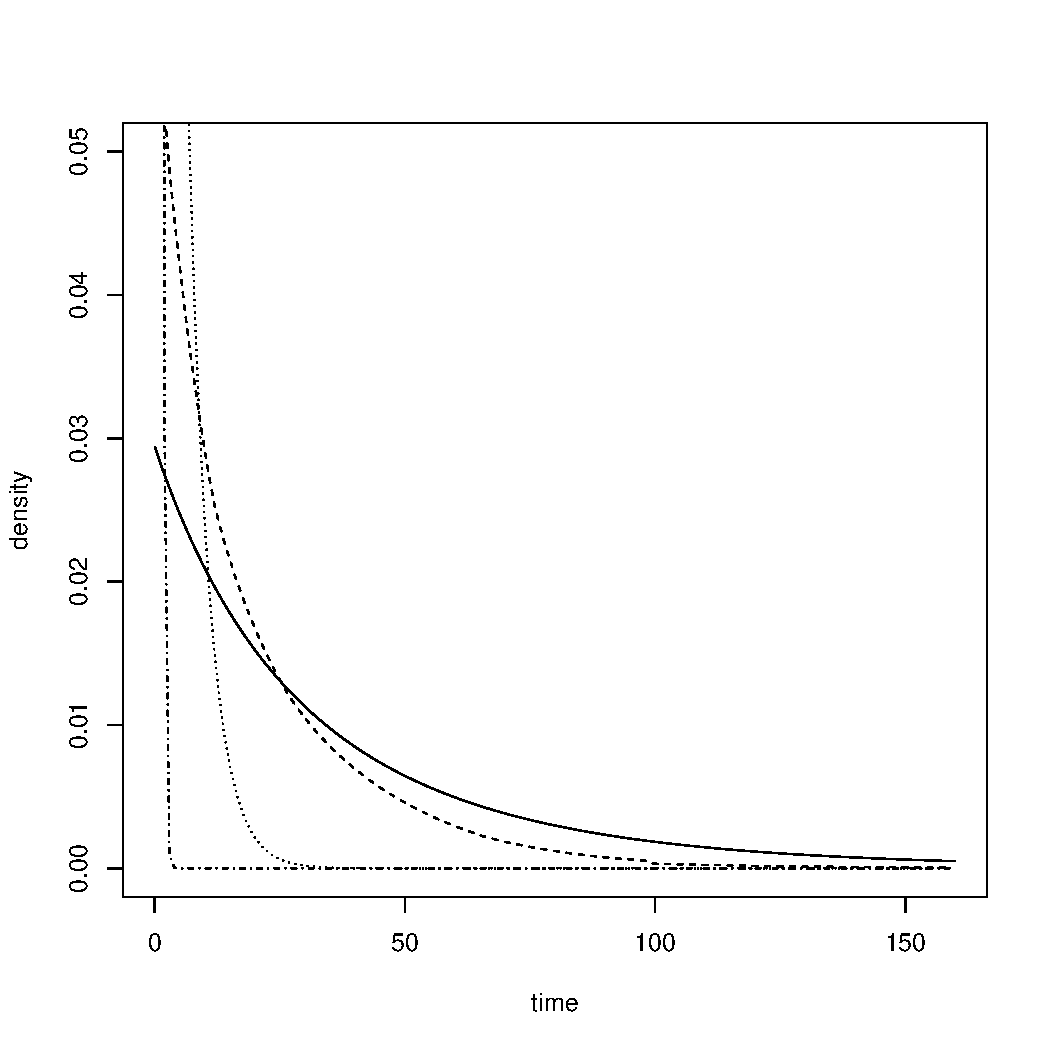
\includegraphics[width=0.6\textwidth]{../priors.pdf}
\label{Fig:Prior}
\end{figure}

\small{Prior density for sampling times under fossilized birth-death process. Dot-dashed line uses priors from \textcite{gavryushkina2015bayesian}. 
Solid line is new prior with implicit assumptions on $T$ and $s$, dashed line results from only assuming implicit prior on $T$,  dotted line results from only assuming implicit prior on $s$.}
\end{frame}



%%%%%%%%%%%%%%%%%%%%%%%%%%%%%%%%%%%%%%%%%%%%%%
\section{Fossil dating}
%%%%%%%%%%%%%%%%%%%%%%%%%%%%%%%%%%%%%%%%%%%%%%

\begin{frame}{And what about this guy?}
\includegraphics[width=0.5\textwidth]{Homo_naledi.jpg}
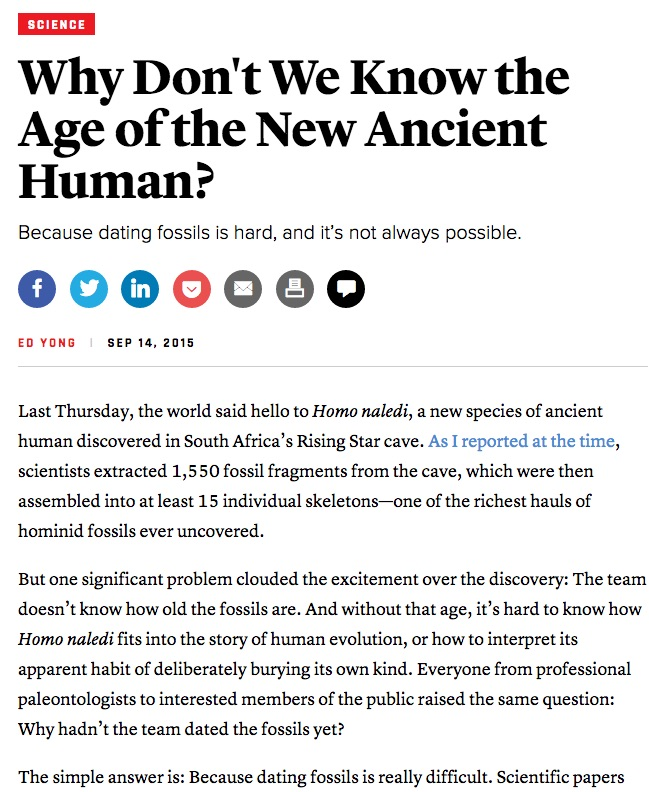
\includegraphics[width=0.5\textwidth]{Atlantic_Homo_naledi.jpg}

\bigskip{}



\end{frame}

\begin{frame}{Can we date fossils using Bayesian phylogenetics? }

Given:
\begin{itemize}
\item A reference set of fossils of known age, and
\item A morphological characterization for reference fossils, and
\item The fossilized birth-death model of sampled ancestor trees
\item A ``clock-like'' model of morphological evolution 
\item A morphological characterization of a related focal fossil of unknown age 
\end{itemize}

{\bf Can the age of the focal fossil be estimated using Bayesian phylogenetic inference?}

\medskip{}

We tested this hypothesis by using the penguin data set. For each of the 36 fossils in turn, we discarded the age information of the focal fossil to mimic the scenario where the age was unknown, and sought to estimate its age using the reference 35 fossils as the reference set. 

\end{frame}


\begin{frame}{Estimating the phylogenetic age of a fossil}
\begin{figure}
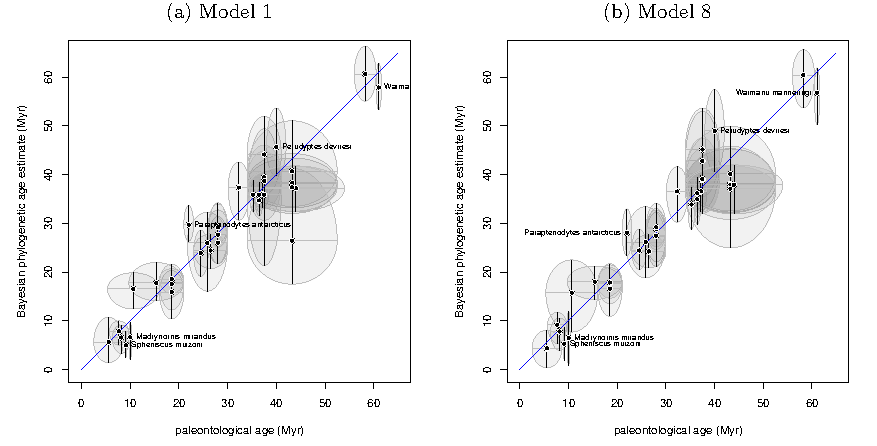
\includegraphics[width=\textwidth]{../Figure1.pdf}
\end{figure}
Bayesian phylogenetic age estimates for each of 36 penguin fossils plotted against their palaeontological age estimates, under two alternative evolutionary models. 
The blue line shows the $x=y$. If the vertical line doesn't cross $x=y$, then the midpoint of the geological range is not in the phylogenetic 95\% HPD. 
\end{frame}

\begin{frame}
\begin{figure}
\includegraphics[width=\textwidth]{../8_penguins_eNprior/8_fossilDatingHist_younger_wide.pdf}
\end{figure}
Marginal posterior density plots for the phylogenetic age estimate of each of the 18 penguin fossils younger than 30 Myr using \Mrelaxed{}. Red boxes are the superimposed age ranges derived from geological data.
\end{frame}

\begin{frame}
\begin{figure}
\includegraphics[width=\textwidth]{../8_penguins_eNprior/8_fossilDatingHist_older_wide.pdf}
\end{figure}
Marginal posterior density plots for the phylogenetic age estimate of each of the 18 penguin fossils older than 30 Myr using \Mrelaxed{}. Red boxes are the superimposed age ranges derived from geological data.
\end{frame}

\begin{frame}
\begin{figure}
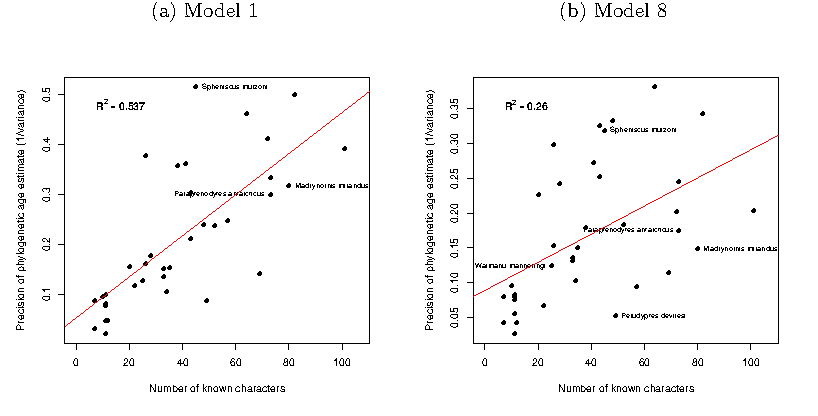
\includegraphics[width=\textwidth]{../Figure2.pdf}
\end{figure}
A plot of the number of non-ambiguous morphological sites for the taxon against the precision of the phylogenetic age for (a) \Mstrict{} and (b) \Mrelaxed{} (i.e. the precision is 1/variance in the marginal posterior distribution of the age).
\end{frame}

\begin{frame}
\frametitle{Comparison of age \& BF estimates between models}
\begin{figure}%
\centering
\subfigure[Estimated phylogenetic age of \Mstrict{} against \Mrelaxed{}.]{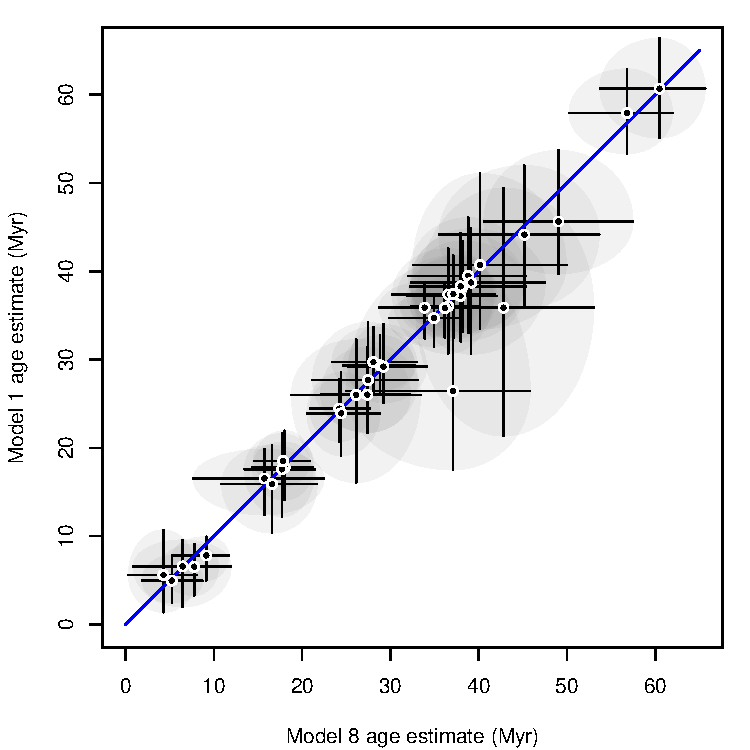
\includegraphics[width=0.45\textwidth]{../compareAgeM1M8.pdf}}\qquad
\subfigure[Regression of Bayes factor (BF) for palaeontological range of \Mstrict{} against \Mrelaxed{}.]{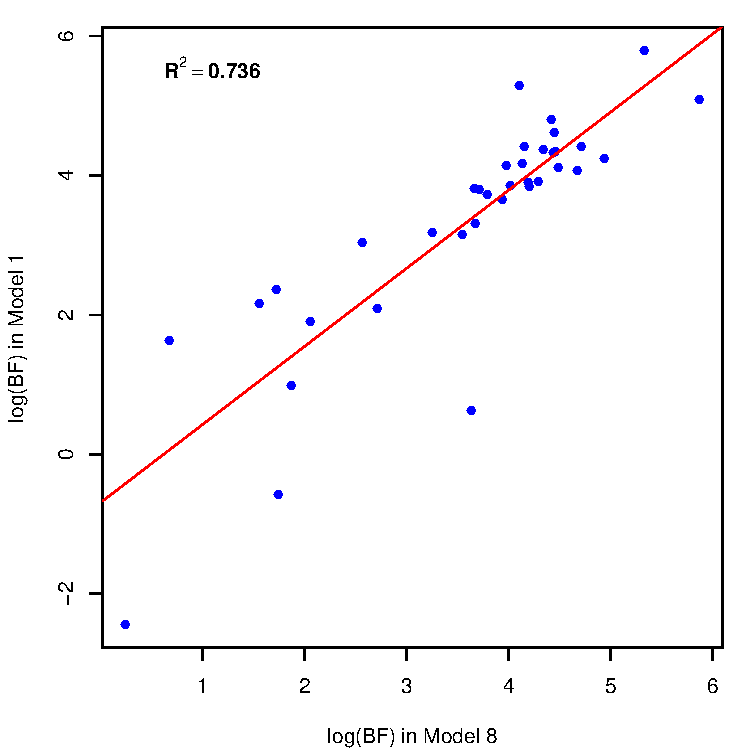
\includegraphics[width=0.45\textwidth]{../compareBFM1M8.pdf}}\\
\label{fig:compareM1M8ab}
\end{figure}
\end{frame}

\begin{frame}
\frametitle{Comparison of probability \& error between models}
\begin{figure}%
\centering
\subfigure[Regression of posterior probability of palaeontological range of \Mstrict{} against \Mrelaxed{}.]{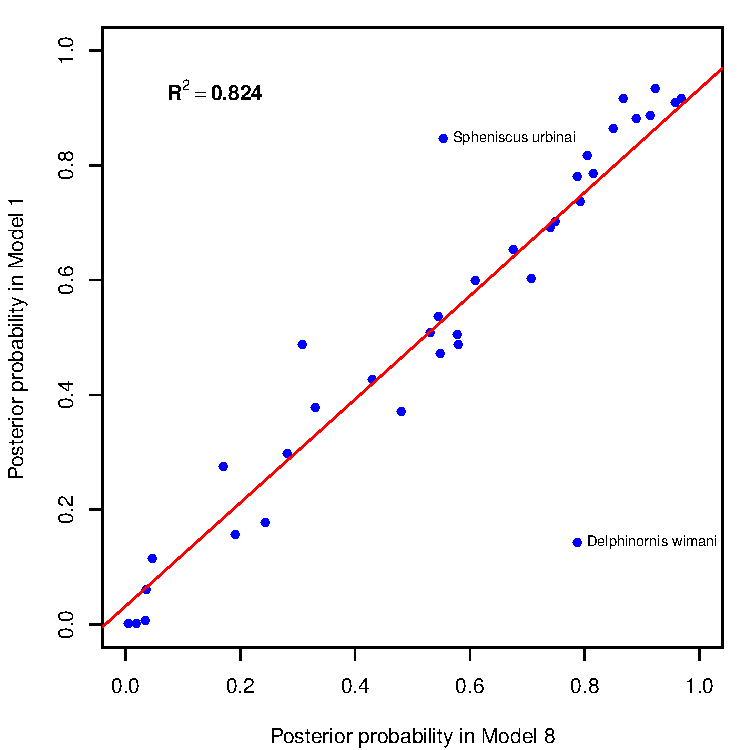
\includegraphics[width=0.45\textwidth]{../comparePostM1M8.pdf}}\qquad
\subfigure[Regression of error in estimated phylogenetic age of \Mstrict{} against \Mrelaxed{}.]{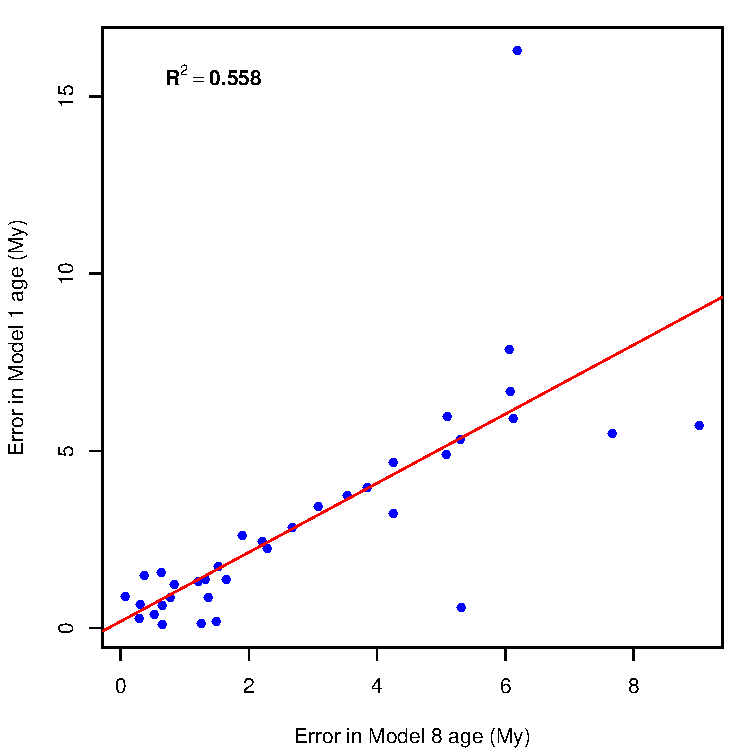
\includegraphics[width=0.45\textwidth]{../compareErrorM1M8.pdf}}\\
\label{fig:compareM1M8cd}
\end{figure}
\end{frame}


%%%%%%%%%%%%%%%%%%%%%%%%%%%%%%%%%%%%%%%%%%%%%%
\section{Canids}
%%%%%%%%%%%%%%%%%%%%%%%%%%%%%%%%%%%%%%%%%%%%%%

\begin{frame}
\begin{figure}
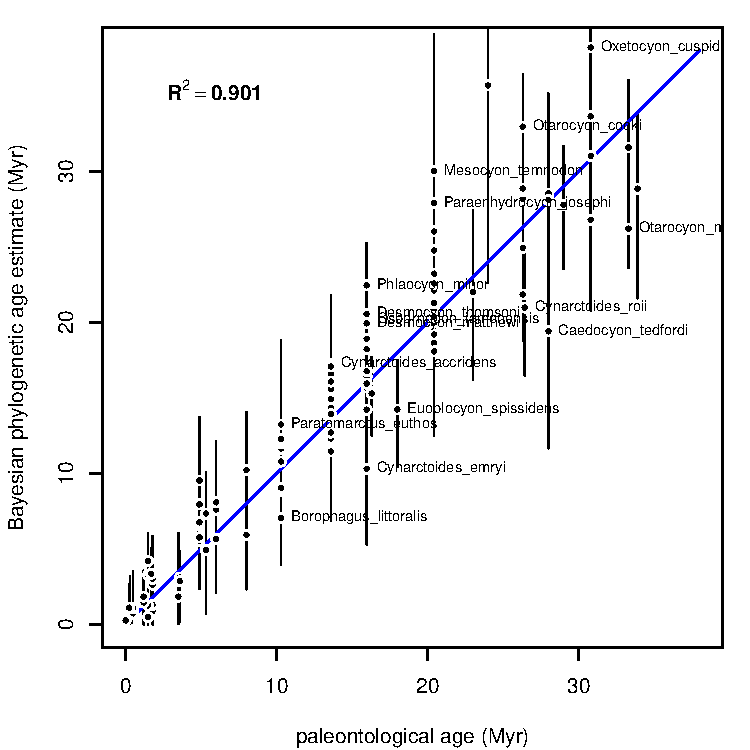
\includegraphics[width=0.70\textwidth]{../canids/1c_phyloAgeVsGeoAge.pdf}
\end{figure}
{\small Bayesian phylogenetic ages for each of 123 canid fossils plotted against palaeontological ages, under \Mstrict{}. 
Bayesian estimates are represented by the median and the 99\% HPD interval of posterior. Blue line shows the $x=y$. 
16 fossils with inconsistent estimates are labelled.}
\end{frame}

%%%%%%%%%%%%%%%%%%%%%%%%%%%%%%%%%%%%%%%%%%%%%%

\begin{frame}
\begin{figure}
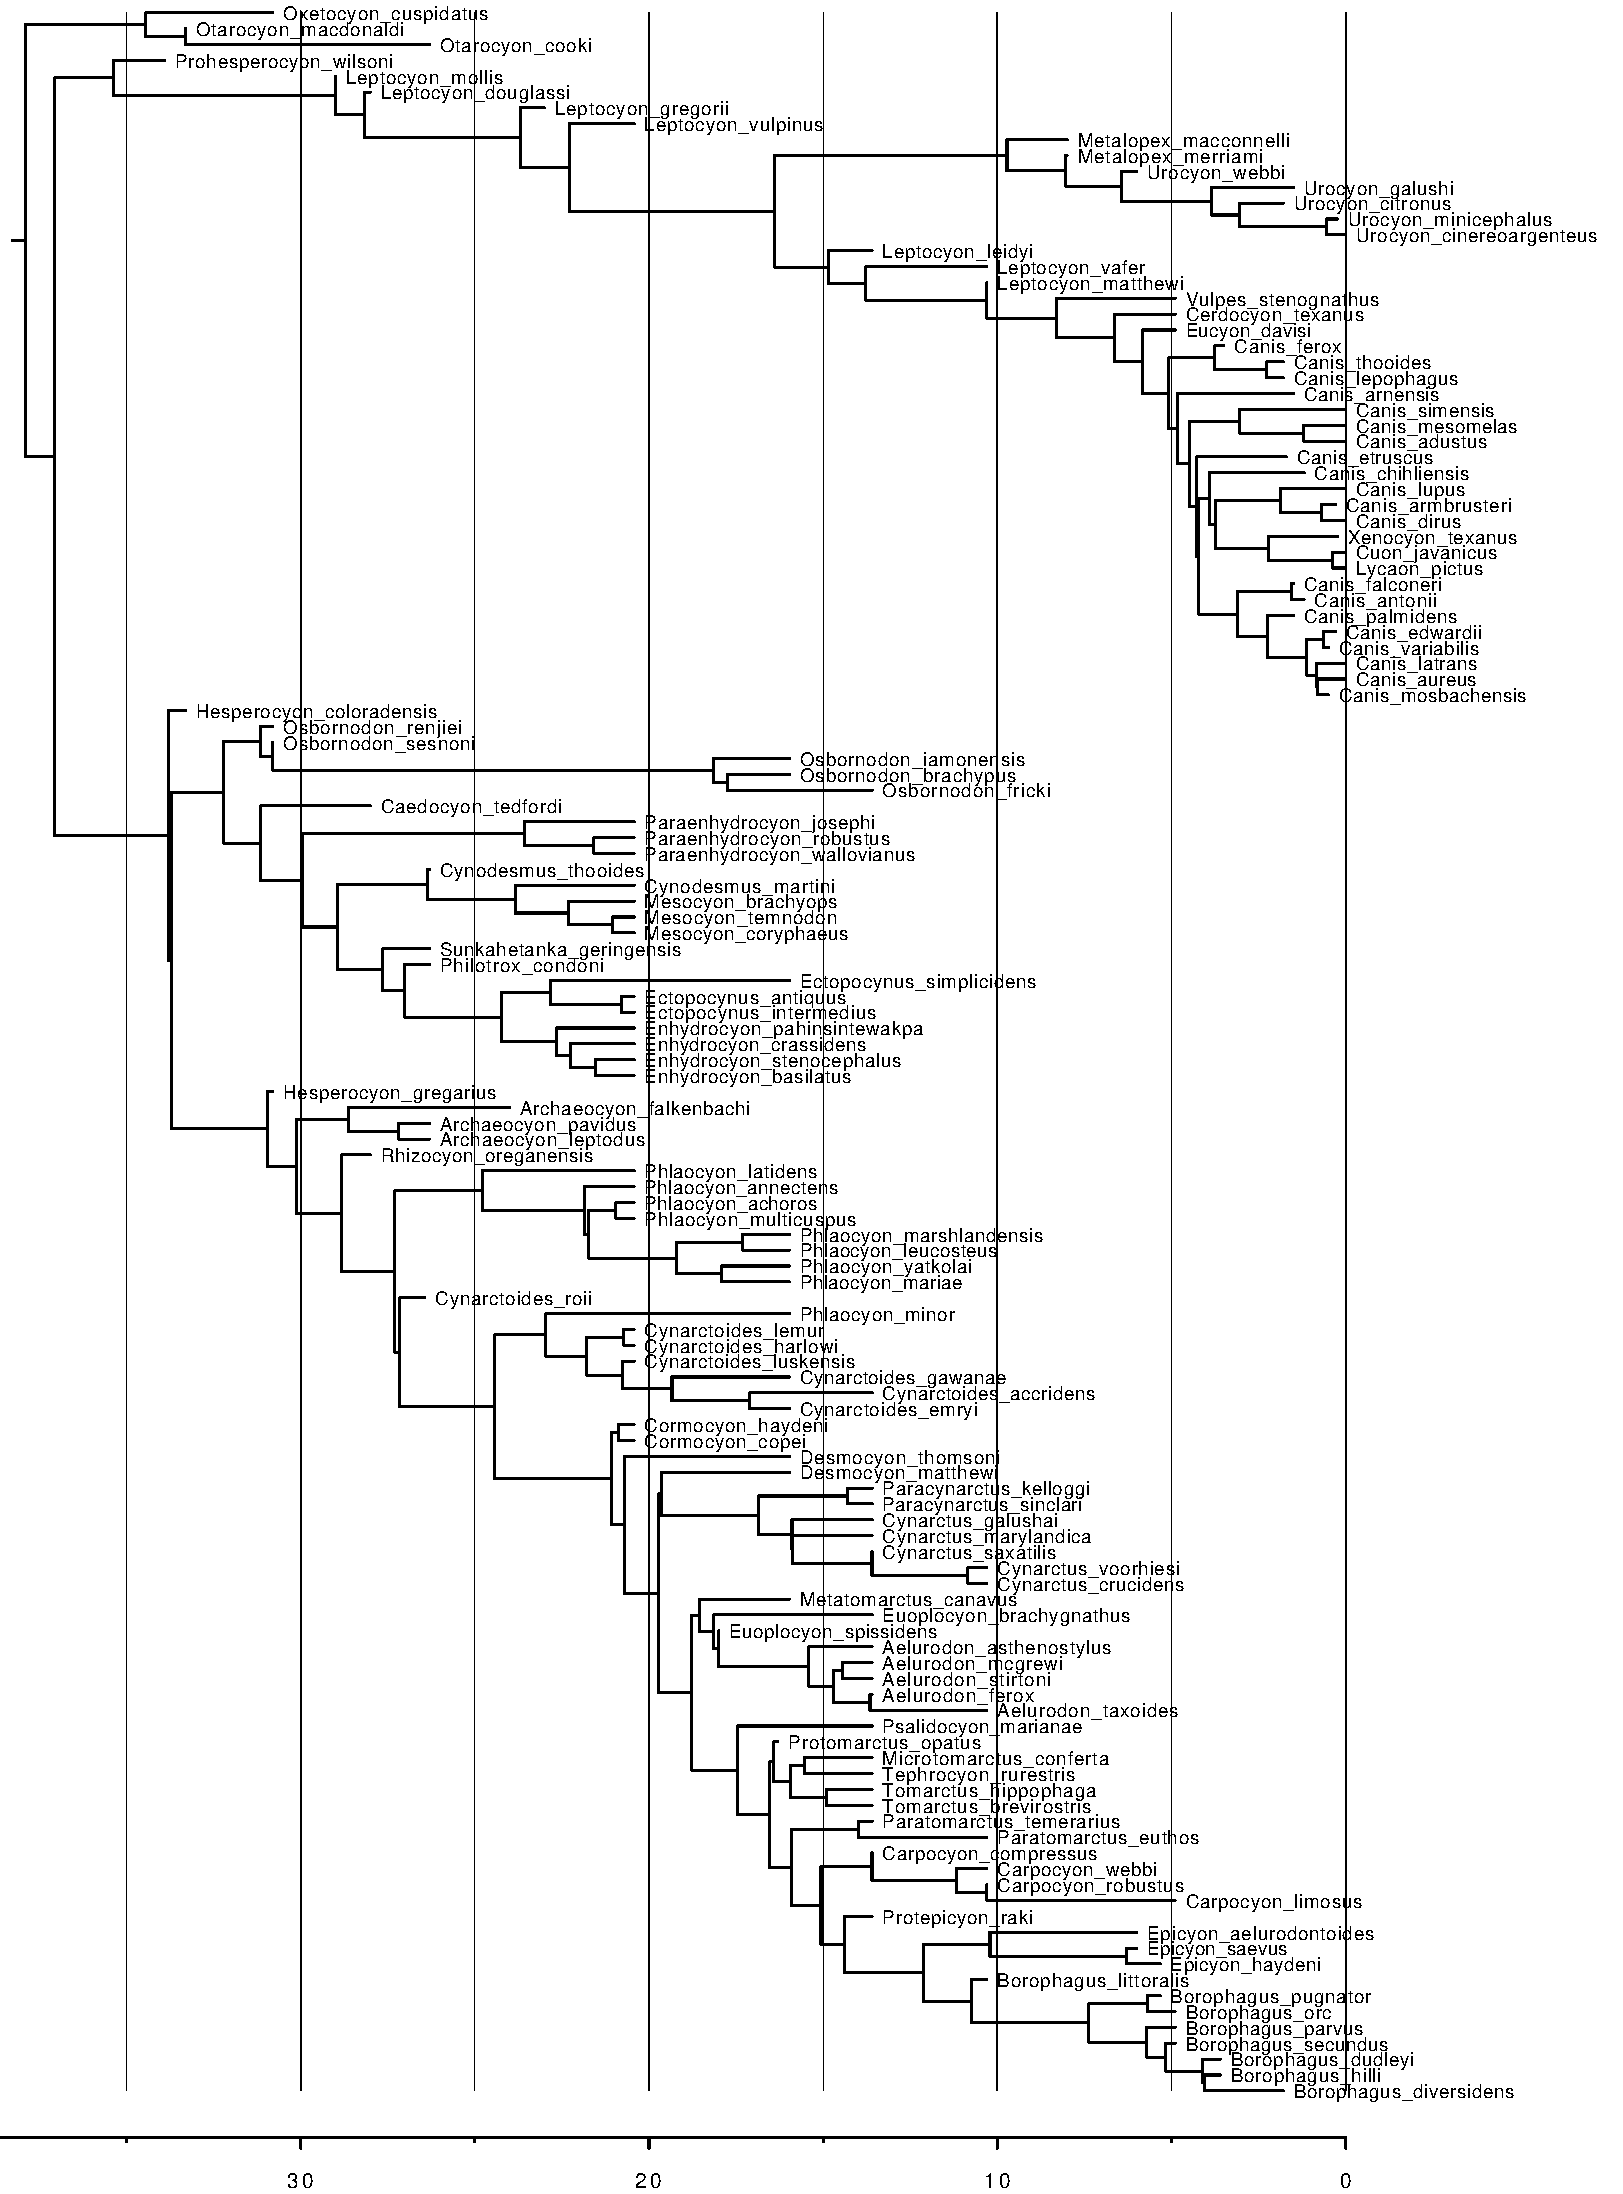
\includegraphics[width=0.5\textwidth]{../canids/1_canids-1440516016976-tree5001.pdf}
\end{figure}
A sample from the posterior distribution of an analysis of the canid data set, showing two main clades, one containing the extant taxa and another constituted entirely of extinct fossil species.
\end{frame}


%%%%%%%%%%%%%%%%%%%%%%%%%%%%%%%%%%%%%%%%%%%%%%
\section{Hominins}
%%%%%%%%%%%%%%%%%%%%%%%%%%%%%%%%%%%%%%%%%%%%%%

\begin{frame}
\frametitle{Controversies in human evolution: {\it Ardipithecus ramidus}}
\begin{figure}
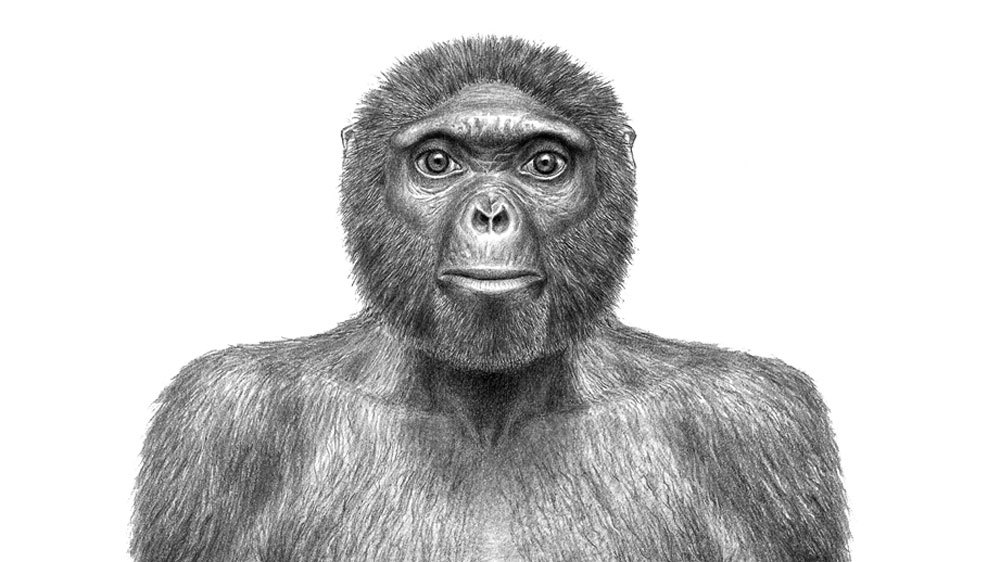
\includegraphics[width=\textwidth]{ardi_crop.jpg}
\end{figure}
`Ardi', 4.4M years old was described as a the oldest fossil relative on the human lineage, a {\it hominin}, and thus more closely related to the human than the chimpanzee. 
\end{frame}

\begin{frame}{Hominin phylogeny inferred using FBD tree prior \& morphological clock.}
\begin{figure}
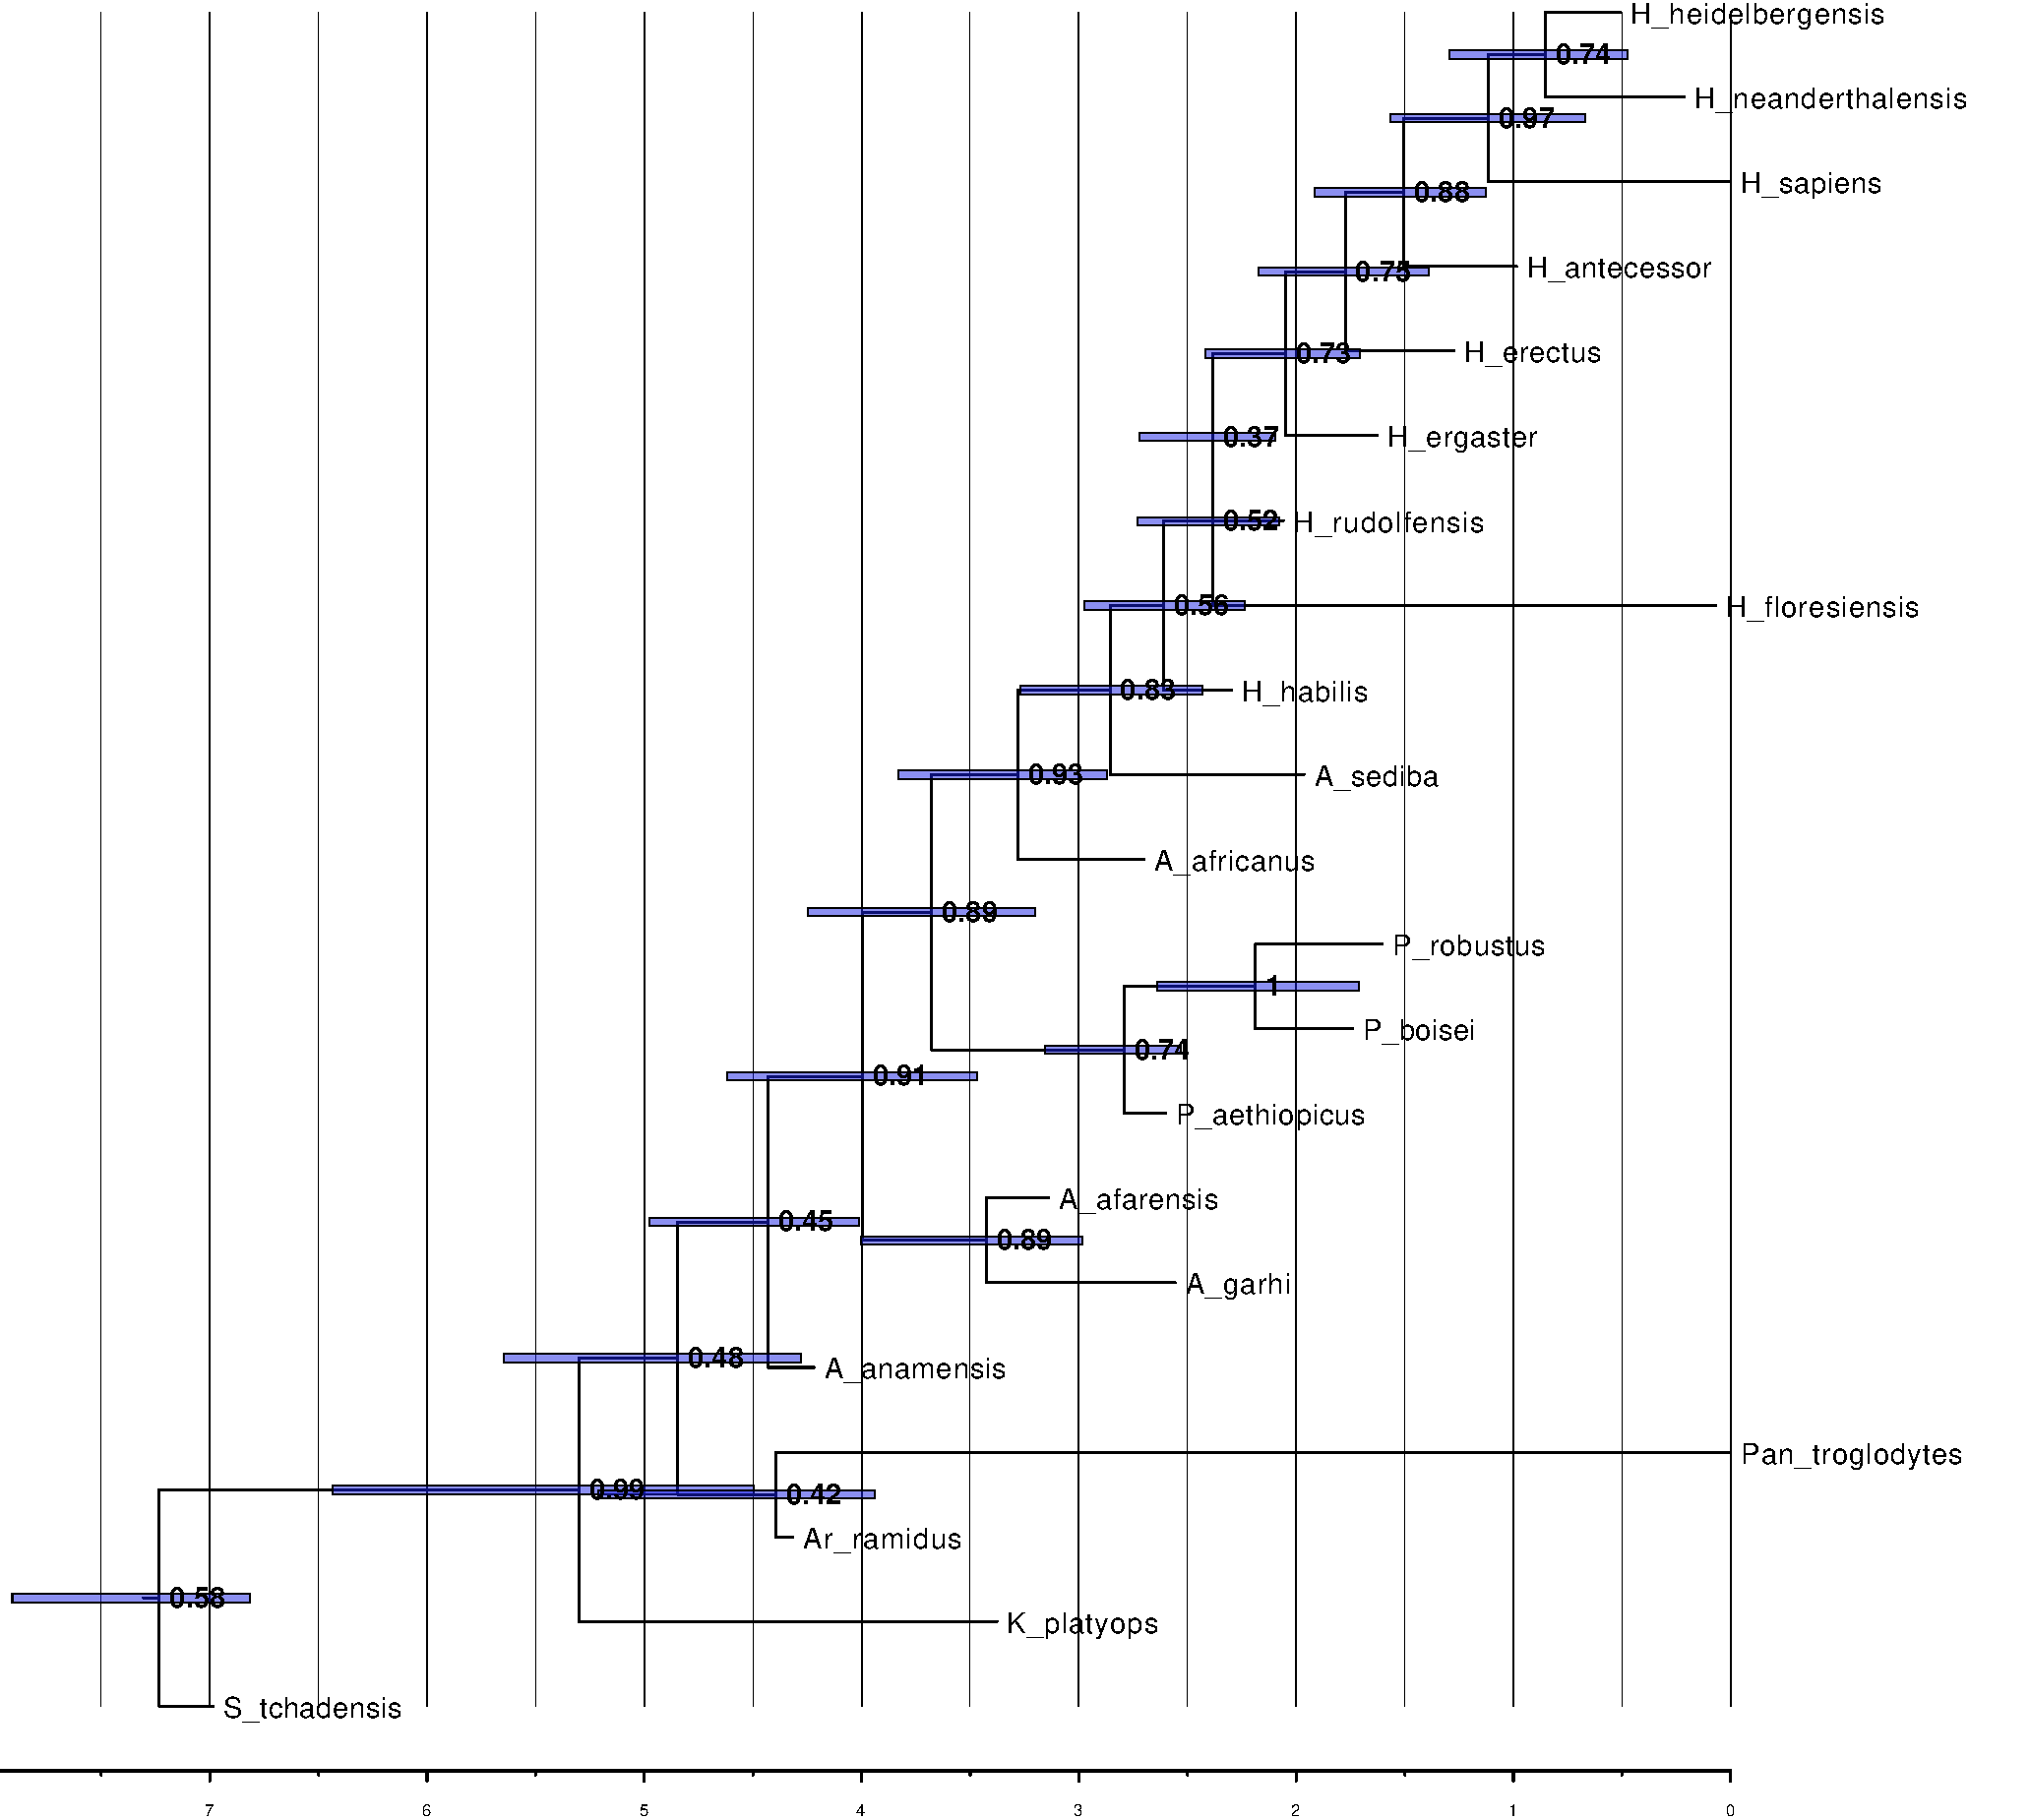
\includegraphics[width=0.75\textwidth]{homininSummaryTree.pdf}
\end{figure}
\end{frame}


%%%%%%%%%%%%%%%%%%%%%%%%%%%%%%%%%%%%%%%%%%%%%%
\section{Conclusions}
%%%%%%%%%%%%%%%%%%%%%%%%%%%%%%%%%%%%%%%%%%%%%%


\begin{frame}{Conclusions and Future Directions}

\begin{itemize}
\item FBD (skyline) is an elegant solution to the divergence dating problem
\item Bayesian inference implementations of FBD on sampled ancestor trees are already quite computationally tractable
\item The effects of hyper parameter priors need to be examined carefully
\item The {\bf morphological clock hypothesis seems adequate} to estimate fossil ages in a range of well-characterized fossil data sets.
\item Summarizing sampled ancestor trees is more complicated and more work on summary and visualization are needed.
\item Improved models of fossilization, speciation and extinction are obvious candidates for future work.
\end{itemize}

\end{frame}

\begin{frame}{Acknowledgements}
\begin{itemize}
\item Sasha Gavryushkina, University of Auckland
\item Tanja Stadler, ETH
\item David Welch, University of Auckland
\item Tracy Heath, Iowa State University
\item Daniel Ksepka, Bruce Museum, Greenwich
\end{itemize}
\end{frame}

\end{document}
